\section{Realisierung}
\label{sec:Realisierung}

Wie im Anhang (\secref{sec:Entscheidung-Programmiersprache}) beschrieben und begründet, wird \texttt{px} mit \textsc{Go} umgesetzt. Da die Standard Library von \textsc{Go} sehr umfassend ist, die mit dem Package \texttt{net/http} über einen mächtigen HTTP-Client (und Server) verfügt, wird nur eine Fremdkomponente (Zugriff auf den Keystore) eingesetzt.

Enorm hilfreich in der Umsetzung war Standardwerk zu \textsc{Go} \cite{gopl}, das nicht nur die Programmiersprache beschreibt, sondern auch deren idiomatischen Gebrauch.

\subsection{Architektur}

\textsc{Go}-Code wird in sogenannte Packages aufgeteilt. Da das Projekt in \textsc{GitLab} \texttt{px} heisst, wird das Hauptpackage als \texttt{px} benannt. Im Root-Verzeichnis befindet sich kein \textsc{Go}-Code.\footnote{\texttt{px.go} beinhaltet bloss eine Package-Deklaration mit einem entsprechenden Kommentar.} Dieser ist in verschiedenen Unterverzeichnissen (\texttt{requests}, \texttt{tokenstore}, usw.) abgelegt. Die Dateien in den Unterpackages deklarieren ihre Packagezugehörigkeit jeweils mit dem unmittelbaren Überverzeichnis, also beispielsweise nicht \texttt{px/tokenstore}, sondern nur \texttt{tokenstore}. Bei der Verwendung der Packages hingegen wird der ganze Pfad angegeben: \texttt{px/tokenstore}.

Der Code für das ausführbare Programm (\texttt{px.go}) befindet sich gemäss Konvention\footnote{\url{https://github.com/golang-standards/project-layout\#cmd}} im \texttt{cmd}-Unterverzeichnis \cite[S. 12]{powerful-cli-apps-in-go}. Das Package heisst jedoch nicht \texttt{cmd}, sondern \texttt{main}, und verfügt über eine Funktion namens \texttt{main} als Haupteinstiegspunkt. Somit ist \texttt{px} als Library, und \texttt{cmd/px.go} als Client dieser Library zu verstehen.\footnote{Da sich nur knapp ein Viertel des Programmcodes im Client-Teil befinden, könnte auf Basis der \texttt{px}-Library recht einfach ein alternativer Client umgesetzt werden.} Die Projektstruktur ist auf der linken Seite der \imgref{img:Komponentendiagramm} zu sehen. Die einzelnen Packages haben folgende Verantwortlichkeiten:

\begin{figure}
    \centering
    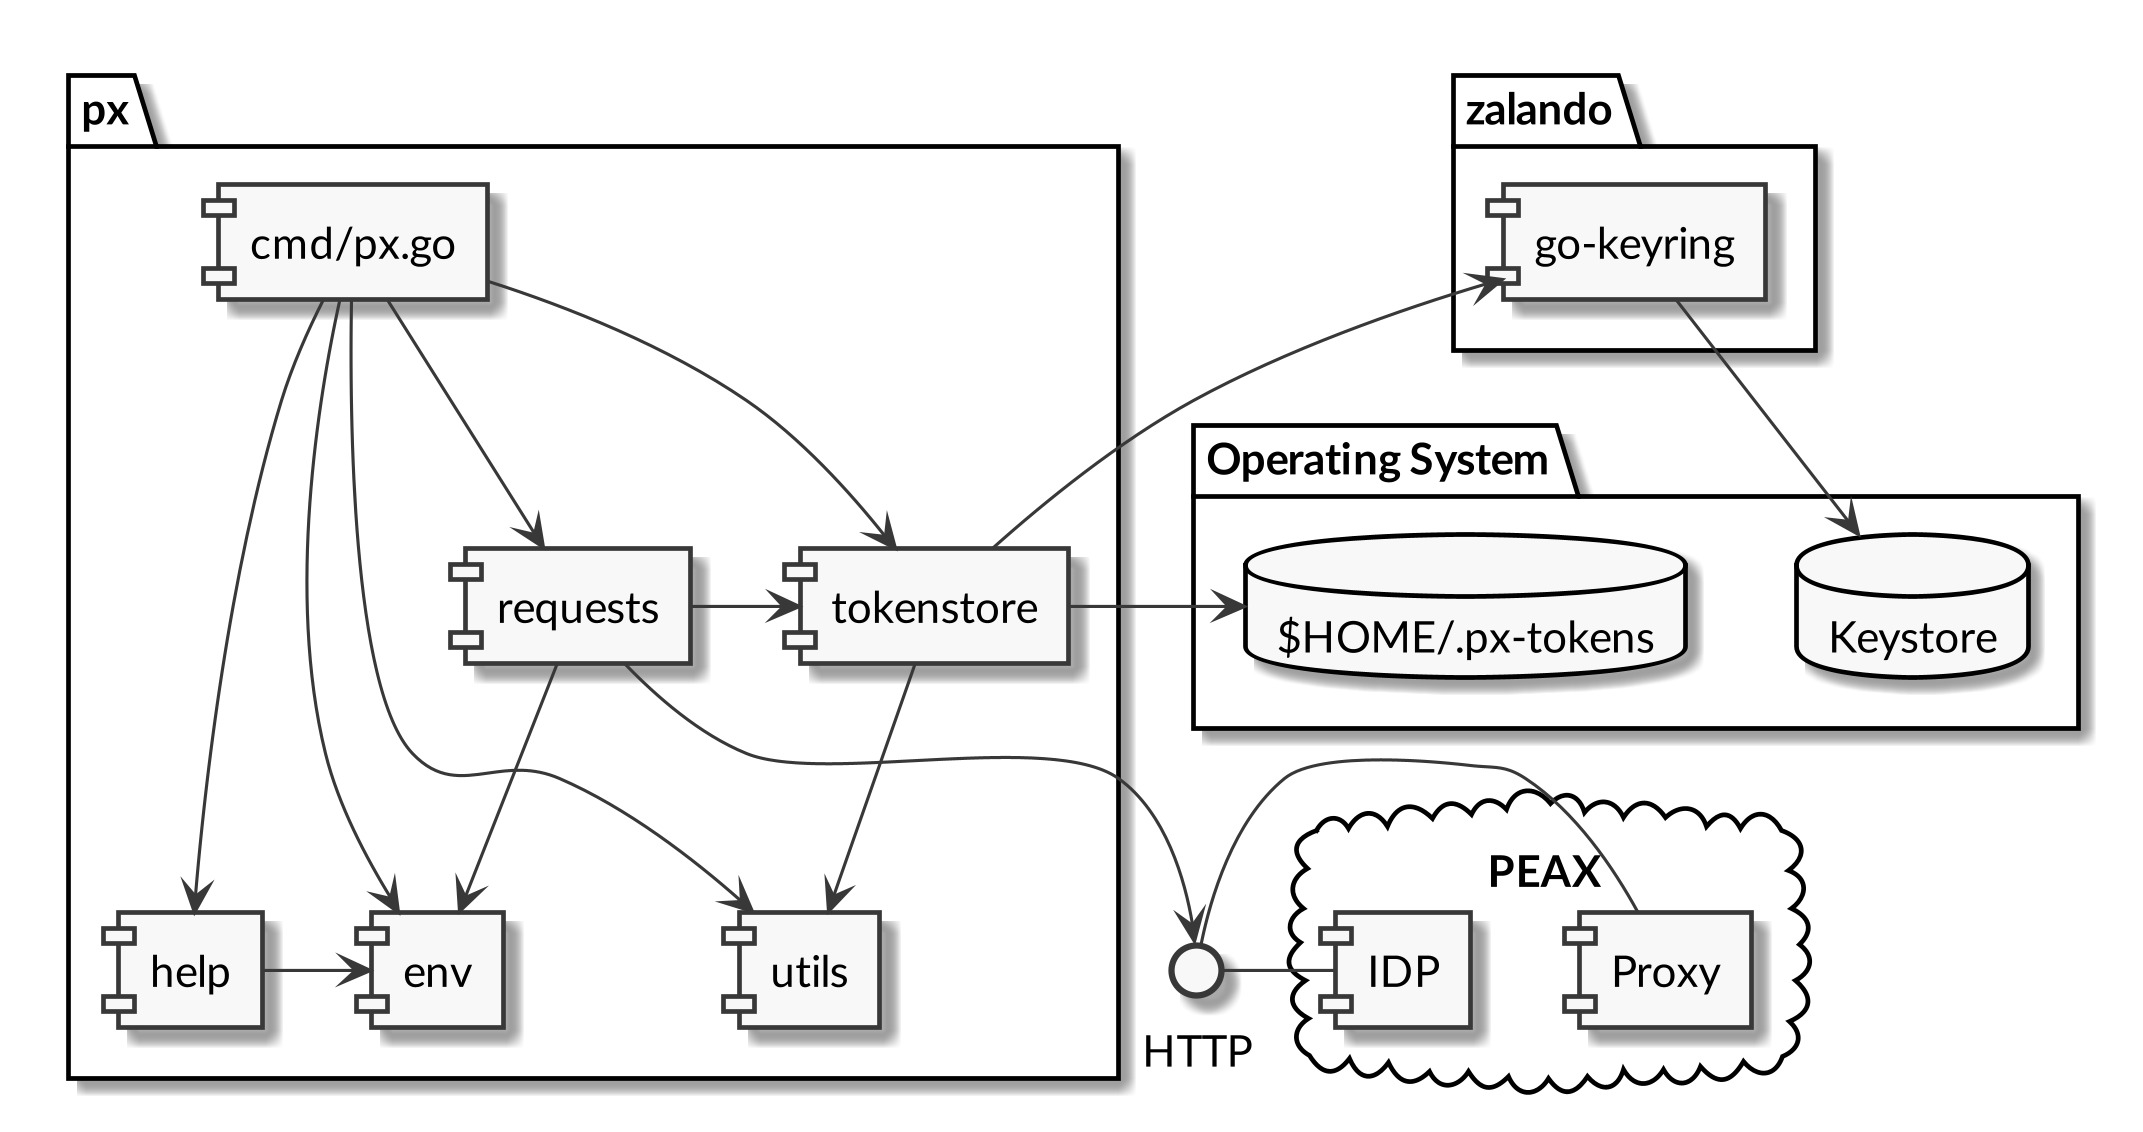
\includegraphics[width=\linewidth]{pics/komponentendiagramm.png}
    \caption{Komponentendiagramm: Die Komponentenarchitektur von \texttt{px}}
    \label{img:Komponentendiagramm}
\end{figure}

\begin{description}
    \item[\texttt{env}] Die Umgebungen (\secref{sec:Umgebungen}) sind in diesem Package aufgelistet. Jede Umgebung verfügt über ein URL-Schema, womit (via Proxy) auf das Backend und direkt auf den IDP zugegriffen werden kann. Verschiedene Funktionen bieten die Möglichkeit, URLs für den Ressourcenzugriff anhand der jeweiligen Umgebung und weiterer Parameter zu erzeugen, was mit dem Unit Test \texttt{env\_test.go} überprüft wird. Die Standardeinstellung, welcher Keystore (sicher/unsicher) zu verwenden ist, wird statisch pro Umgebung definiert.
    \item[\texttt{help}] Dieses Package umfasst die Hilfetexte. Zu jedem Befehl gibt es jeweils eine kurze, einzeilige Beschreibung, und einen ausführlichen Hilfetext. Dieses Package importiert das \texttt{env}-Package, damit bei der Hilfe zum Login-Befehl (\texttt{px login}) die verfügbaren Umgebungen automatisch aufgelistet werden können.
    \item[\texttt{tokenstore}] TODO: Abbilden der Datenstruktur, Extraktion von Informationen, JSON-(Un)marshaling
    \item[\texttt{requests}] TODO: Retry-Mechanismus, Funktion für jede Methode, Hilfsfunktionen
    \item[\texttt{utils}] TODO: Filesystem, Terminal Input
    \item[\texttt{cmd/px.go}] TODO: Map mit Key=Command, Value=(Hilfetexte, Funktion) beschreiben
\end{description}

\subsection{Zwei-Faktor-Authentifizierung}

\begin{figure}
    \centering
    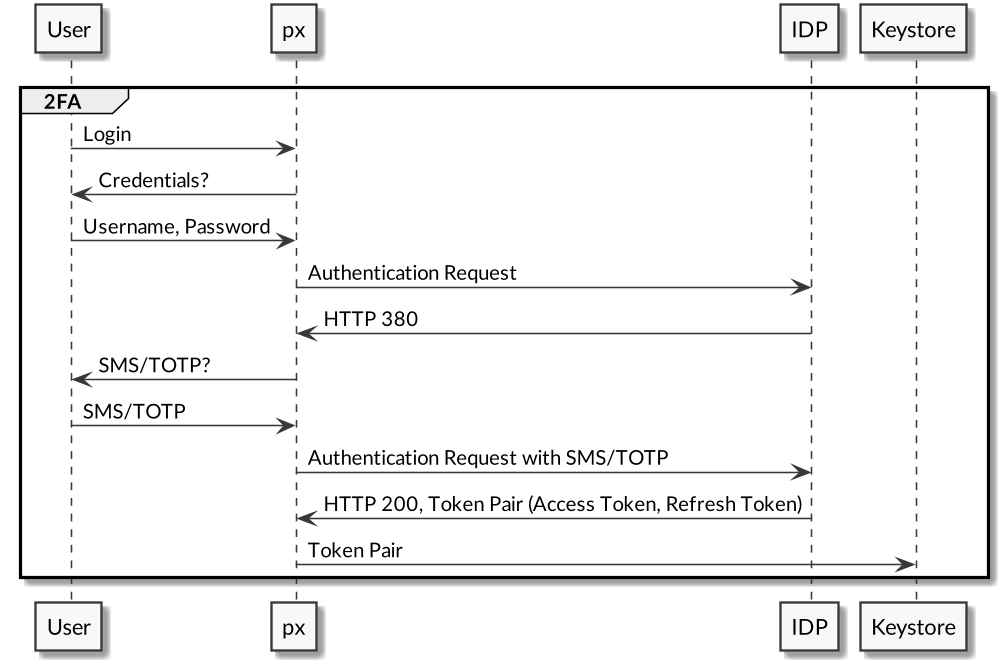
\includegraphics[width=\linewidth]{pics/sequence-2fa.png}
    \caption{Sequenzdiagramm: Der Ablauf der Zwei-Faktor-Authentifizierung mit SMS oder OTP}
\end{figure}

\subsection{Token Store}
\label{sec:Realisierung-Token-Store}

TODO: sicher und unsicher, Datenstruktur

\subsubsection{Fremdkomponente \texttt{zalando/go-keyring}}

\subsection{Retry-Mechanismus}
\label{sec:Retry-Mechanismus}

\begin{figure}
    \centering
    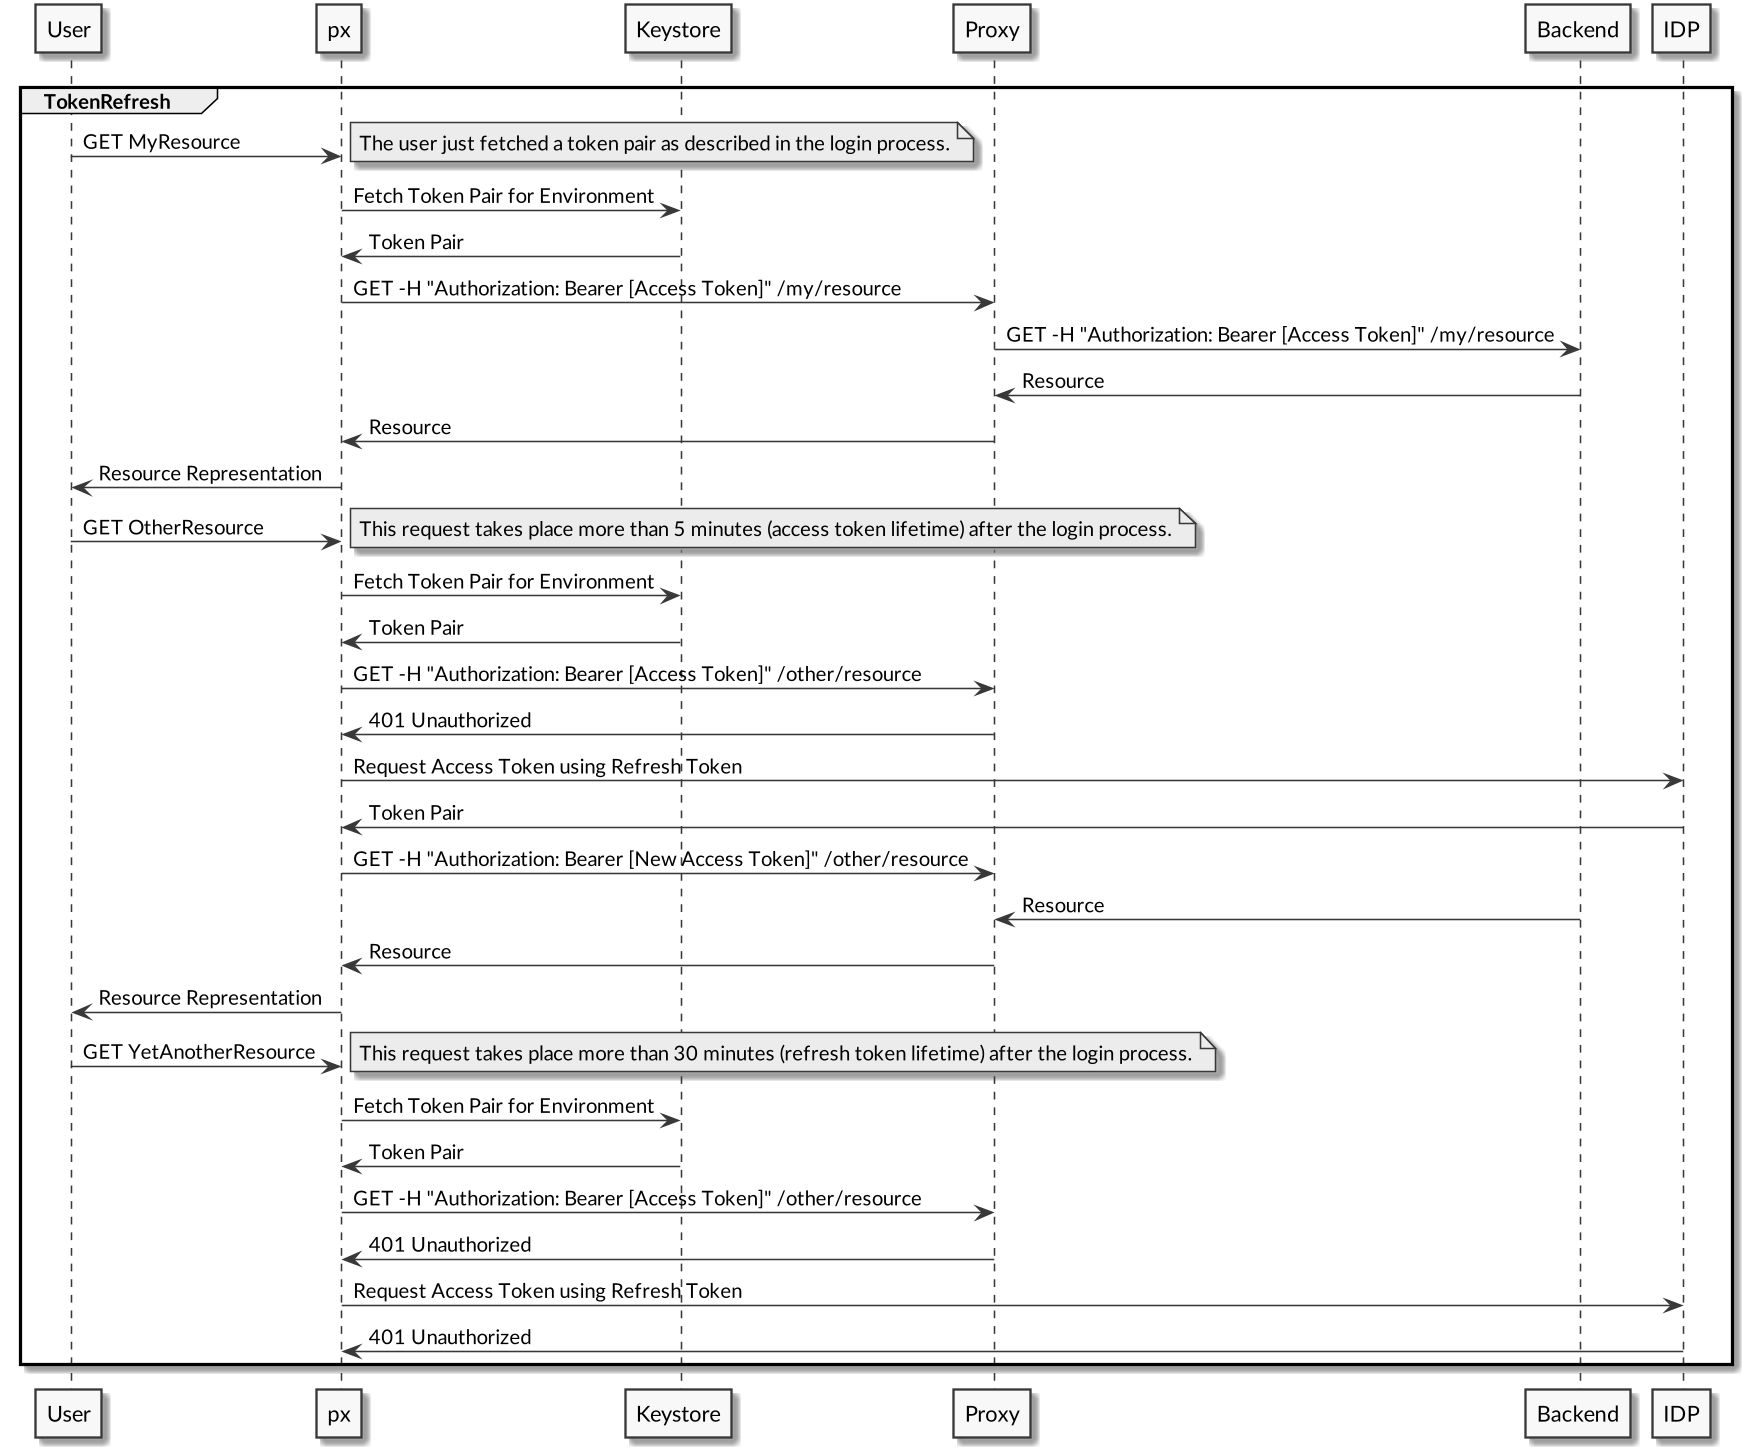
\includegraphics[width=\linewidth]{pics/sequence-retry.png}
    \caption{Sequenzdiagramm: Der für den Benutzer transparente Retry-Mechanismus mit einem Token Pair, das im Hintergrund automatisch aktualisiert wird}
\end{figure}
